% ============================================================
\chapter{Syst\`emes Lin\'eaires et Classification des Portraits de Phase}
\label{ch:lineaires}
% ============================================================

\section{Introduction}

Avant d'affronter les tourbillons du chaos et la complexit\'e des syst\`emes non lin\'eaires, il faut ma\^itriser le cas lin\'eaire --- celui o\`u tout peut \^etre calcul\'e explicitement. Le portrait de phase d'un syst\`eme lin\'eaire plan est enti\`erement d\'etermin\'e par les valeurs propres de sa matrice~: n\oe uds stables ou instables, foyers spiralants, centres elliptiques, points-selles. Cette classification, h\'erit\'ee des travaux de Poincar\'e et de son \'el\`eve Ivar Bendixson \`a la fin du XIX\textsuperscript{e} si\`ecle, constitue le dictionnaire visuel que tout dynamicien consulte en premier.

Mais le syst\`eme lin\'eaire n'est pas qu'un exercice p\'edagogique. Gr\^ace au th\'eor\`eme de Hartman-Grobman, le portrait de phase lin\'earis\'e autour d'un \'equilibre hyperbolique reproduit fid\`element le comportement local du syst\`eme non lin\'eaire. C'est pourquoi les syst\`emes lin\'eaires constituent la brique \'el\'ementaire de la th\'eorie
des syst\`emes dynamiques. Ce chapitre d\'eveloppe la
classification compl\`ete des portraits de phase pour les syst\`emes plans
$\dot{x} = Ax$, $x \in \R^2$.

\section{Solution g\'en\'erale et exponentielle de matrice}

\begin{theoreme}[Solution du syst\`eme lin\'eaire]
La solution du syst\`eme $\dot{x} = Ax$ avec condition initiale $x(0) = x_0$
est
\[
    x(t) = e^{At}\, x_0,
\]
o\`u l'\textbf{exponentielle de matrice} est d\'efinie par
\[
    e^{At} = \sum_{k=0}^{+\infty} \frac{(At)^k}{k!} = I + At + \frac{A^2 t^2}{2!} + \cdots
\]
\end{theoreme}

\begin{proposition}[Propri\'et\'es de $e^{At}$]
\begin{enumerate}
    \item $e^{A \cdot 0} = I$ ;
    \item $\frac{d}{dt} e^{At} = A e^{At} = e^{At} A$ ;
    \item $e^{A(t+s)} = e^{At}\, e^{As}$ ;
    \item $(e^{At})^{-1} = e^{-At}$ ;
    \item Si $P$ est inversible, $e^{(P^{-1}AP)t} = P^{-1} e^{At} P$ ;
    \item $\det(e^{At}) = e^{\mathrm{tr}(A)\, t}$.
\end{enumerate}
\end{proposition}

\begin{formules}[title=\textbf{Calcul de $e^{At}$ pour $A \in \R^{2 \times 2}$}]
Si $A$ a pour valeurs propres $\lambda_1, \lambda_2$ :
\begin{itemize}
    \item \textbf{Cas $\lambda_1 \neq \lambda_2$ r\'eelles} :
    $e^{At} = \frac{\lambda_2 e^{\lambda_1 t} - \lambda_1 e^{\lambda_2 t}}{\lambda_2 - \lambda_1} I
    + \frac{e^{\lambda_2 t} - e^{\lambda_1 t}}{\lambda_2 - \lambda_1} A$.
    \item \textbf{Cas $\lambda_1 = \lambda_2 = \lambda$} :
    $e^{At} = e^{\lambda t}(I + (A - \lambda I)t)$ si $A \neq \lambda I$.
    \item \textbf{Cas complexes $\lambda = \alpha \pm i\beta$} :
    $e^{At} = e^{\alpha t}\left(\cos(\beta t)\, I + \frac{\sin(\beta t)}{\beta}(A - \alpha I)\right)$.
\end{itemize}
\end{formules}

\section{Classification dans $\R^2$}

Consid\'erons le syst\`eme $\dot{x} = Ax$ o\`u $A \in \R^{2\times 2}$ et
$\det(A) \neq 0$ (l'origine est l'unique point d'\'equilibre). Les invariants
pertinents sont :
\begin{itemize}
    \item $\tau = \mathrm{tr}(A) = \lambda_1 + \lambda_2$ ;
    \item $\delta = \det(A) = \lambda_1 \lambda_2$ ;
    \item $\Delta = \tau^2 - 4\delta$ (discriminant du polyn\^ome caract\'eristique).
\end{itemize}

\subsection{N\oe ud stable ($\lambda_1 < \lambda_2 < 0$)}

\begin{definition}[N\oe ud stable]
Le portrait de phase est un \textbf{n\oe ud stable} lorsque les deux valeurs
propres sont r\'eelles et strictement n\'egatives. Toutes les orbites
convergent vers l'origine tangentiellement au sous-espace propre associ\'e \`a
la valeur propre de plus grand module.
\end{definition}

Conditions : $\delta > 0$, $\tau < 0$, $\Delta > 0$.

\begin{center}
\begin{tikzpicture}
    \begin{axis}[
        width=7cm, height=7cm,
        xlabel={$x_1$}, ylabel={$x_2$},
        xmin=-3, xmax=3, ymin=-3, ymax=3,
        axis lines=middle, ticks=none,
        title={N\oe ud stable}
    ]
    % Trajectories toward origin
    \addplot[blue, thick, ->, domain=0:2.5, samples=50] ({2.5*exp(-x)*cos(30)}, {2.5*exp(-2*x)*sin(30)});
    \addplot[blue, thick, ->, domain=0:2.5, samples=50] ({-2*exp(-x)*cos(20)}, {2*exp(-2*x)*sin(50)});
    \addplot[blue, thick, ->, domain=0:2.5, samples=50] ({1.5*exp(-x)}, {-2*exp(-2*x)});
    \addplot[blue, thick, ->, domain=0:2.5, samples=50] ({-2*exp(-x)}, {-1.5*exp(-2*x)});
    \node at (axis cs:0,0) [circle, fill=black, inner sep=1.5pt] {};
    \end{axis}
\end{tikzpicture}
\end{center}

\subsection{N\oe ud instable ($0 < \lambda_1 < \lambda_2$)}

\begin{definition}[N\oe ud instable]
Portrait de phase sym\'etrique du n\oe ud stable : les orbites divergent
de l'origine. Conditions : $\delta > 0$, $\tau > 0$, $\Delta > 0$.
\end{definition}

\subsection{Point col ($\lambda_1 < 0 < \lambda_2$)}

\begin{definition}[Point col]
Le portrait de phase est un \textbf{point col} (ou \textbf{selle}) lorsque
les valeurs propres sont de signes oppos\'es. Les orbites s'approchent de
l'origine le long du sous-espace propre stable et s'en \'eloignent le long
du sous-espace propre instable.
\end{definition}

Conditions : $\delta < 0$.

\begin{center}
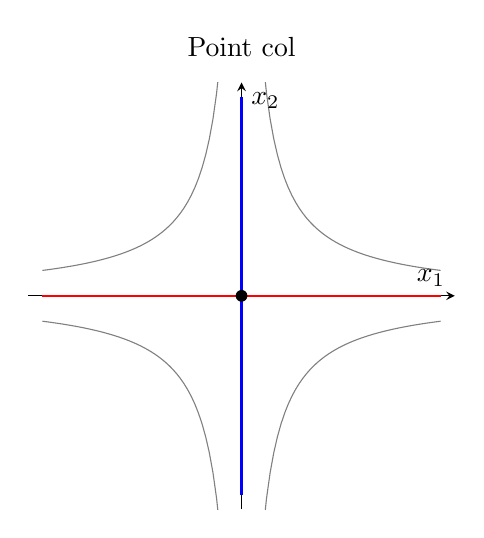
\begin{tikzpicture}
    \begin{axis}[
        width=7cm, height=7cm,
        xlabel={$x_1$}, ylabel={$x_2$},
        xmin=-3, xmax=3, ymin=-3, ymax=3,
        axis lines=middle, ticks=none,
        title={Point col}
    ]
    % Stable and unstable manifolds
    \addplot[red, thick, domain=-2.8:2.8, samples=2] {0};
    \addplot[blue, thick, domain=-2.8:2.8, samples=50] ({0}, {x});
    % Hyperbolic trajectories
    \addplot[gray, domain=0.3:2.8, samples=50] {1/x};
    \addplot[gray, domain=0.3:2.8, samples=50] {-1/x};
    \addplot[gray, domain=-2.8:-0.3, samples=50] {1/x};
    \addplot[gray, domain=-2.8:-0.3, samples=50] {-1/x};
    \node at (axis cs:0,0) [circle, fill=black, inner sep=1.5pt] {};
    \end{axis}
\end{tikzpicture}
\end{center}

\subsection{Foyer stable ($\lambda = \alpha \pm i\beta$, $\alpha < 0$)}

\begin{definition}[Foyer stable]
Le portrait de phase est un \textbf{foyer stable} lorsque les valeurs propres
sont complexes conjugu\'ees \`a partie r\'eelle n\'egative. Les orbites
spiralent vers l'origine.
\end{definition}

Conditions : $\Delta < 0$, $\tau < 0$.

\subsection{Foyer instable ($\alpha > 0$)}

Portrait sym\'etrique : spirales divergentes. Conditions : $\Delta < 0$, $\tau > 0$.

\subsection{Centre ($\lambda = \pm i\beta$, $\alpha = 0$)}

\begin{definition}[Centre]
Le portrait de phase est un \textbf{centre} lorsque les valeurs propres sont
purement imaginaires. Les orbites sont des ellipses ferm\'ees autour de l'origine.
L'\'equilibre est stable mais non asymptotiquement stable.
\end{definition}

Conditions : $\Delta < 0$, $\tau = 0$.

\begin{attention}[title=\textbf{Centre et perturbations non lin\'eaires}]
Un centre lin\'eaire est \emph{structurellement instable} : une perturbation
non lin\'eaire arbitrairement petite peut le transformer en foyer
(stable ou instable). C'est un cas critique de la lin\'earisation.
\end{attention}

\subsection{N\oe ud d\'eg\'en\'er\'e et n\oe ud \'etoil\'e}

\begin{definition}[N\oe ud \'etoil\'e]
Si $A = \lambda I$ ($\lambda < 0$), toutes les droites passant par l'origine
sont des orbites : c'est un \textbf{n\oe ud \'etoil\'e stable}.
\end{definition}

\begin{definition}[N\oe ud d\'eg\'en\'er\'e]
Si $A$ a une valeur propre double $\lambda < 0$ avec un seul vecteur propre
(bloc de Jordan), le portrait de phase est un \textbf{n\oe ud d\'eg\'en\'er\'e
stable}. Toutes les orbites sont tangentes au sous-espace propre.
\end{definition}

\section{Diagramme $(\tau, \delta)$}

La classification compl\`ete se r\'esume dans le plan $(\tau, \delta)$ :

\begin{center}
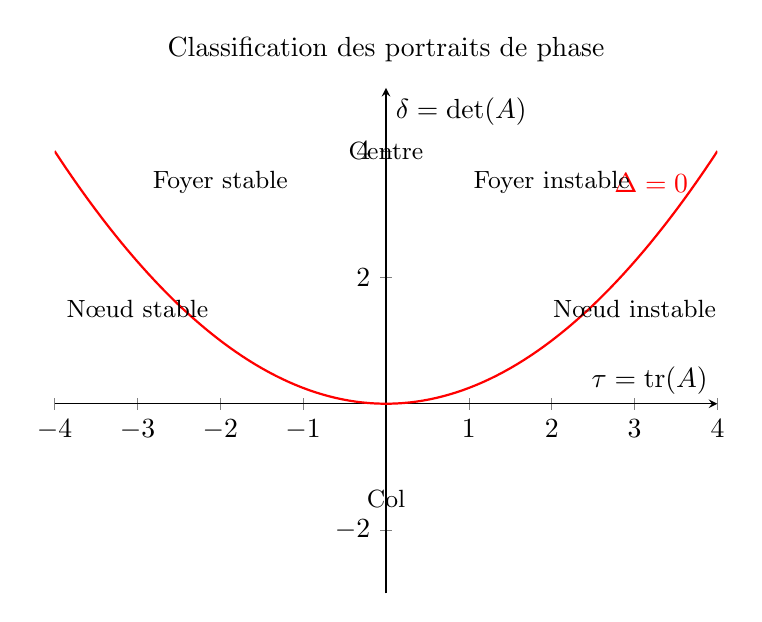
\begin{tikzpicture}
    \begin{axis}[
        width=10cm, height=8cm,
        xlabel={$\tau = \mathrm{tr}(A)$},
        ylabel={$\delta = \det(A)$},
        xmin=-4, xmax=4, ymin=-3, ymax=5,
        axis lines=middle,
        title={Classification des portraits de phase}
    ]
    % Parabola Delta = tau^2/4
    \addplot[thick, red, domain=-4:4, samples=100] {x^2/4};
    \node[red] at (axis cs:3.2,3.5) {$\Delta=0$};
    % Labels
    \node at (axis cs:-2,3.5) {\small Foyer stable};
    \node at (axis cs:2,3.5) {\small Foyer instable};
    \node at (axis cs:0,4) {\small Centre};
    \node at (axis cs:-3,1.5) {\small N\oe ud stable};
    \node at (axis cs:3,1.5) {\small N\oe ud instable};
    \node at (axis cs:0,-1.5) {\small Col};
    \end{axis}
\end{tikzpicture}
\end{center}

\begin{theoreme}[Classification compl\`ete en dimension 2]
Soit $A \in \R^{2\times 2}$ avec $\det(A) \neq 0$. La nature du portrait de
phase de $\dot{x} = Ax$ est enti\`erement d\'etermin\'ee par
$\tau = \mathrm{tr}(A)$ et $\delta = \det(A)$ :
\begin{center}
\begin{tabular}{lll}
\hline
\textbf{Type} & \textbf{Conditions} & \textbf{Stabilit\'e} \\
\hline
N\oe ud stable & $\delta > 0$, $\tau < 0$, $\Delta \geq 0$ & Asymp. stable \\
N\oe ud instable & $\delta > 0$, $\tau > 0$, $\Delta \geq 0$ & Instable \\
Col & $\delta < 0$ & Instable \\
Foyer stable & $\Delta < 0$, $\tau < 0$ & Asymp. stable \\
Foyer instable & $\Delta < 0$, $\tau > 0$ & Instable \\
Centre & $\Delta < 0$, $\tau = 0$ & Stable (non asymp.) \\
\hline
\end{tabular}
\end{center}
\end{theoreme}

\section{Syst\`emes lin\'eaires en dimension sup\'erieure}

\subsection{D\'ecomposition en sous-espaces invariants}

\begin{theoreme}[D\'ecomposition spectrale]
Soit $A \in \R^{n \times n}$. L'espace $\R^n$ se d\'ecompose en somme directe
de sous-espaces invariants :
\[
    \R^n = E^s \oplus E^u \oplus E^c,
\]
o\`u :
\begin{itemize}
    \item $E^s$ (sous-espace \textbf{stable}) : valeurs propres g\'en\'eralis\'ees
    \`a partie r\'eelle $< 0$ ;
    \item $E^u$ (sous-espace \textbf{instable}) : valeurs propres g\'en\'eralis\'ees
    \`a partie r\'eelle $> 0$ ;
    \item $E^c$ (sous-espace \textbf{central}) : valeurs propres g\'en\'eralis\'ees
    \`a partie r\'eelle $= 0$.
\end{itemize}
\end{theoreme}

\begin{proposition}[Comportement asymptotique]
\begin{enumerate}
    \item Pour $x_0 \in E^s$ : $\norm{e^{At} x_0} \to 0$ exponentiellement
    quand $t \to +\infty$.
    \item Pour $x_0 \in E^u$ : $\norm{e^{At} x_0} \to +\infty$ exponentiellement
    quand $t \to +\infty$.
    \item Pour $x_0 \in E^c$ : $\norm{e^{At} x_0}$ cro\^it au plus
    polynomialement.
\end{enumerate}
\end{proposition}

\subsection{Forme de Jordan et exponentielle}

\begin{proposition}[Exponentielle d'un bloc de Jordan]
Si $J_k(\lambda) = \lambda I_k + N_k$ est un bloc de Jordan de taille $k$,
alors
\[
    e^{J_k(\lambda)t} = e^{\lambda t}
    \begin{pmatrix}
        1 & t & \frac{t^2}{2} & \cdots & \frac{t^{k-1}}{(k-1)!} \\
        0 & 1 & t & \cdots & \frac{t^{k-2}}{(k-2)!} \\
        \vdots & & \ddots & & \vdots \\
        0 & 0 & \cdots & 1 & t \\
        0 & 0 & \cdots & 0 & 1
    \end{pmatrix}.
\]
\end{proposition}

\section{Syst\`emes lin\'eaires non autonomes}

\begin{definition}[Matrice fondamentale]
Pour le syst\`eme $\dot{x} = A(t)\, x$, une \textbf{matrice fondamentale}
est une matrice $\Phi(t) \in \R^{n \times n}$ dont les colonnes forment un
syst\`eme fondamental de solutions. Elle satisfait
$\dot{\Phi}(t) = A(t)\, \Phi(t)$ et $\det(\Phi(t)) \neq 0$.
\end{definition}

\begin{theoreme}[Formule de Liouville-Jacobi]
$\det(\Phi(t)) = \det(\Phi(t_0))\, \exp\!\left(\int_{t_0}^t \mathrm{tr}(A(s))\, ds\right)$.
\end{theoreme}

\section{Applications}

\begin{exemple}[Circuit RLC]
Un circuit RLC s\'erie est gouvern\'e par
\[
    L\ddot{q} + R\dot{q} + \frac{q}{C} = 0,
\]
ce qui donne en posant $x_1 = q$, $x_2 = \dot{q}$ :
\[
    A = \begin{pmatrix} 0 & 1 \\ -\frac{1}{LC} & -\frac{R}{L} \end{pmatrix}.
\]
Selon les valeurs de $R$, $L$, $C$ :
\begin{itemize}
    \item $R^2 < 4L/C$ : foyer stable (oscillations amorties) ;
    \item $R^2 = 4L/C$ : n\oe ud d\'eg\'en\'er\'e (amortissement critique) ;
    \item $R^2 > 4L/C$ : n\oe ud stable (sur-amortissement).
\end{itemize}
\end{exemple}

\begin{codeblock}[title=\textbf{Portraits de phase pour diff\'erentes matrices}]
\begin{minted}{python}
import numpy as np
import matplotlib.pyplot as plt
from scipy.integrate import solve_ivp

matrices = {
    "Noeud stable": np.array([[-2, 0], [0, -1]]),
    "Col": np.array([[-1, 0], [0, 1]]),
    "Foyer stable": np.array([[-0.5, 2], [-2, -0.5]]),
    "Centre": np.array([[0, 1], [-1, 0]])
}

fig, axes = plt.subplots(2, 2, figsize=(10, 10))
for ax, (name, A) in zip(axes.flat, matrices.items()):
    for angle in np.linspace(0, 2*np.pi, 20, endpoint=False):
        x0 = 2 * np.array([np.cos(angle), np.sin(angle)])
        sol = solve_ivp(lambda t, x: A @ x, [0, 10], x0,
                        max_step=0.05)
        ax.plot(sol.y[0], sol.y[1], 'b-', lw=0.5)
    ax.set_title(name)
    ax.set_xlim(-3, 3); ax.set_ylim(-3, 3)
    ax.set_aspect('equal'); ax.grid(True, alpha=0.3)
plt.tight_layout()
plt.savefig("phase_portraits_linear.pdf")
plt.show()
\end{minted}
\end{codeblock}

\section{Exercices}

\begin{exercice}[Exponentielle de matrice]
Calculer $e^{At}$ pour $A = \begin{pmatrix} 1 & 1 \\ 0 & 1 \end{pmatrix}$
(bloc de Jordan). Tracer le portrait de phase.
\end{exercice}

\begin{exercice}[Classification]
Classifier le portrait de phase de $\dot{x} = Ax$ pour
\[
    A = \begin{pmatrix} a & 1 \\ -1 & a \end{pmatrix}
\]
en fonction du param\`etre $a \in \R$.
\end{exercice}

\begin{exercice}[Dimension 3]
Trouver les sous-espaces stable, instable et central pour
$A = \begin{pmatrix} -1 & 0 & 0 \\ 0 & 0 & -1 \\ 0 & 1 & 0 \end{pmatrix}$.
\end{exercice}

\begin{exercice}[Syst\`eme p\'eriodique]
Consid\'erer le syst\`eme p\'eriodique $\dot{x} = A(t)x$ avec
$A(t) = \begin{pmatrix} 0 & 1 \\ -\omega^2(t) & 0 \end{pmatrix}$
o\`u $\omega(t) = \omega_0(1 + \epsilon\cos(t))$. Discuter la stabilit\'e
en utilisant la th\'eorie de Floquet.
\end{exercice}

\begin{exercice}[\'Equivalence topologique]
Montrer que deux n\oe uds stables avec des valeurs propres distinctes sont
topologiquement \'equivalents mais pas n\'ecessairement $C^1$-conjugu\'es.
\end{exercice}

\begin{exercice}[Diagramme de stabilit\'e]
Pour le syst\`eme d\'ependant de deux param\`etres
$A = \begin{pmatrix} 0 & 1 \\ -a & -b \end{pmatrix}$,
tracer dans le plan $(a, b)$ les r\'egions correspondant aux diff\'erents
types de portraits de phase.
\end{exercice}
